\documentclass[11pt]{article}
% /usr/local/texlive/2013/bin/x86_64-darwin/pdflatex 
\usepackage[T1]{fontenc}
\usepackage[utf8]{inputenc}
\usepackage[fleqn]{amsmath}
\usepackage{amssymb}
\usepackage{graphicx}
\usepackage{hyperref}
\usepackage{parskip}
\usepackage{tikz} 
\usepackage{wrapfig} 
\usepackage{alltt}

\renewcommand{\ttdefault}{txtt}

\usepackage[letterpaper]{geometry}
\linespread{1.5}
\usepackage[font=small,labelfont=bf]{caption}
%\usepackage{cancel}

% körper und mengen
\newcommand{\setn}{\mathbb N}
\newcommand{\setr}{\mathbb R}
\newcommand{\setc}{\mathbb C}
\newcommand{\setk}{\mathbb K}

% reihe von #1 bis unendlich über #2
\newcommand{\reihe}[2]{\sum\limits_{#1}^{\infty}{#2}}
% summe von #1 bis #2 über #3
\newcommand{\summe}[3]{\sum\limits_{#1}^{#2}{#3}}
% integral von #1 bis #2 über #3 nach #4
\newcommand{\integrald}[4]{\int\limits_{#1}^{#2}{#3 \; \mathrm d#4}}
% integral von #1 bis #2 über #3 (d/dx muss dann selbst angegeben werden)
\newcommand{\integral}[3]{\int\limits_{#1}^{#2}{#3}}
% integralberechnung von #1 bis #2 über 3
\newcommand{\integralv}[3]{\left[ #3 \right]_{#1}^{#2}}
% betrag mit wachsenden betragsstrichen
\newcommand{\betrag}[1]{\left| #1 \right|}
% limes n gegen unendlich
\newcommand{\limesn}[1]{\lim\limits_{n \to \infty}{#1}}
% limes h gegen 0
\newcommand{\limesh}[1]{\lim\limits_{h \to 0}{#1}}
% vektor kurzschreibweise...
\newcommand{\vect}[1]{\left(\begin{array}{c}#1\end{array}\right)}
%normen
\newcommand{\norm}[1]{\left \Vert {#1} \right \Vert}
\newcommand{\normzwei}[1]{\norm {#1}_{2}}
\newcommand{\norminfty}[1]{\norm {#1}_{\infty}}
\newcommand{\qed}{\hfill \ensuremath{\Box}}
% namentabelle till lukas stefan
\newcommand{\lukas}{\begin{center}
	\begin{tabular}{c|c}
		Name & Student ID \\
		\hline
		Lukas Pfahler & 577332 \\
	\end{tabular}
\end{center}}
% gruppe
\newcommand{\gruppe}[1]{\begin{center} Gruppe {#1} \end{center}}

\title{Information Retrieval and Web Search - Project Phase 1}
\author{Lukas Pfahler \and Tejas Umakanth}
\begin{document}
\maketitle
\section{Collaboration Details}
	We both do everything. clever...asdfa sdkfjalöksdj fölakdjf öaljdf,ajhdf a abdf afas
	dasfdghalkjdhfa


	adsfadsf

	sfg
	asd
\section{Description}
	\begin{wrapfigure}[5]{l}{3.15cm}
  		\vspace{-0.6cm}
  		
\includegraphics[width=3.4cm,height=3.4cm]{logo.png}
	\end{wrapfigure}
	For our project, we decided to crawl and index data found on Instagram\footnote{\url{http://instagram.com}}. Instagram is a popular\footnote{Instagram reported 150 million users in September, 2013.} social media application that allows users to publish photos and videos and search the media published by other users. Each user is identified by a unique user name. Each media item can have a caption, a list of comments by other users or a location. As known from other popular social networks like Twitter and Facebook, captions and comments can contain hashtags.
\section{Architecture}
	\subsection{Crawler}
		Instagram offers a developer API that allows us to subscribe to real time updates and crawl new media items as soon as they are posted.\footnote{\url{http://instagram.com/developer/realtime/}} There are different options for subscriptions: You can either subscripe to a specific user, hashtag or to a geographic area or location. All communication between the crawler and instagram is done using the HTTP protocol: The crawler is itself a http-server and once we subscripe to media updates at instagram.com, their servers start connecting to our crawler. Everytime there is new media, they issue a http POST request. The post does not contain the actual media, but is merely a notification that there has been an update. We then grab the actual data by requesting all recently added media from their servers in a http GET request.

		\vspace{0.5cm}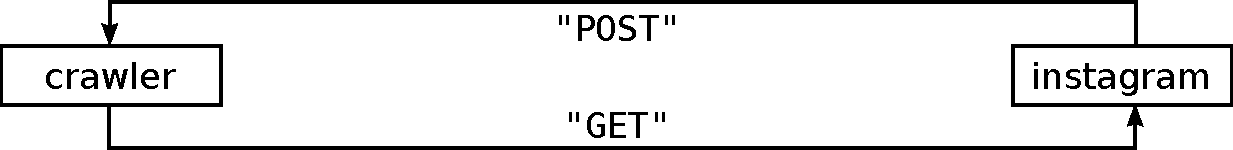
\includegraphics[width=\textwidth,keepaspectratio]{crawler.pdf}

		The response is a JSON file containing a list of media items. We save each of those items in a separate JSON file. We also save a 150$\times$150px jpeg thumbnail image for each media item.

		Our crawler is based on the software platform Node.js, which allows us to setup a http-server and request data in an asynchronous fashion with very little javascript code.
		\begin{quote}
			Node.js is a platform built on Chrome's JavaScript runtime. [..] It uses an event-driven, non-blocking I/O model that makes it lightweight and efficient, perfect for data-intensive real-time applications that run across distributed devices.\footnote{\url{http://nodejs.org/}}
		\end{quote}

		Instagram allowes developers to issue 5000 requests per hour\footnote{\url{http://instagram.com/developer/endpoints/}}, thus we introduced a politeness factor $p$: Only every $p$-th time our crawler is notified we actually request the new data. This has three effects: First, the number of requests is reduced and second, the number of new media items per response is higher. It also means that we probably miss a fraction of the data. However, if one would setup a larger system with multiple crawlers the coverage would increase. Third, for subscriptions with a very high update frequency, this makes sure we don't try to download more than our own bandwidth limit allows us to.

	\subsection{Indexing}
		A problem with the data crawled from Instagram is, that it contains only a relatively small amount of caption text - oftentimes the caption is merely a list of hashtags. To get more text, we index a concatenation of the caption and all comments. If the item is supplied with a named location, we also add the name to the indexed text. We call this concatenation $body$. From $body$ we remove all $\#$-characters. If the crawler subscribed to a specific hashtag, we also remove this tag, since it is present in all items and thus is useless for indexing.

		Furthermore, we introduce a field just for indexing the list of hashtags provided to the media item. Note that this are both hashtags from the caption and from the comments. Also we index the username separately.

		Finally, we use Lucene's spatial indexing module to index the media items by their GPS locations. Internally, this builds a inverted index based on Geohash\footnote{See \url{http://en.wikipedia.org/wiki/Geohash} for more details}. The spatial module hashes longitude/latitude points to strings, such that close points share a longer prefix. It then builds a prefix tree on those strings and builds a inverted index of its nodes.

\section{Usage}
	\subsection{Crawler}
		To run our crawler, you first have to install node.js, which you can download at 
		\begin{center}{\vspace{-3mm}\url{http://nodejs.org/download/}}\end{center}
		We are also using the request node-module, which you can download and install by running the following command:
		\begin{alltt}
			npm install request
		\end{alltt}
		Now you can run our crawler by calling
		\begin{alltt}
			node instagramStream.js
		\end{alltt}
		which will start a http-server on port 1337 of your local machine. Please note that port 1337 of your machine has to be open to the public. To actually start crawling, you have to subscribe to instagram media updates. This is done by calling the following command:
		\begin{alltt}
			curl -F 'client_id=620c46f7e7da46149b0ad5d3cd8268ba' \textbackslash 
			     -F 'client_secret=c57beab5c2864e608b0dc4e46e5f8b50' \textbackslash
			     -F 'object=tag' -F 'aspect=media' -F 'object_id=\textbf{selfie}' \textbackslash
			     -F 'callback_url=\{http://\textbf{YOUR_IP}:1337\}' \textbackslash
			     https://api.instagram.com/v1/subscriptions/
		\end{alltt}
		This will subscribe to all updates of the (very popular) hashtag $\#$selfie; the crawler will start storing media items in a newly created folder selfies.

		You can unsubscribe from updates by running
		\begin{alltt}
			curl -X DELETE 'https://api.instagram.com/v1/subscriptions?client_secret=\textbackslash
			     c57beab5c2864e608b0dc4e46e5f8b50&object=all&\textbackslash
			     client_id=620c46f7e7da46149b0ad5d3cd8268ba'
		\end{alltt}

		You should always unsubscribe before shutting down the crawler (\texttt{CTRL-C}), if you fail to do so you might not be able to subscribe to media for a while. We suspect that the servers at Instagram need some time to realize that our crawler is not running anymore and continue to try to send the new subscriptions to our already shutdown crawler.
	\subsection{Indexer}
\section{Performance}
	The time needed to for indexing is dependant on the system on which the indexing is done. This performance analysis was carried out on a laptop with a 2.4 GHz CPU. For performing this test, we use a document containing 3GB worth of JSON files that are returned by our crawler. Then we try to index 10k,20k and so on up to 50k JSON files in the document and calculate the time taken to index in each case. As we can see in figure~\ref{fig:1}, the indexing time increases almost linearly as the number of files that are indexed increases.
	\begin{figure}
		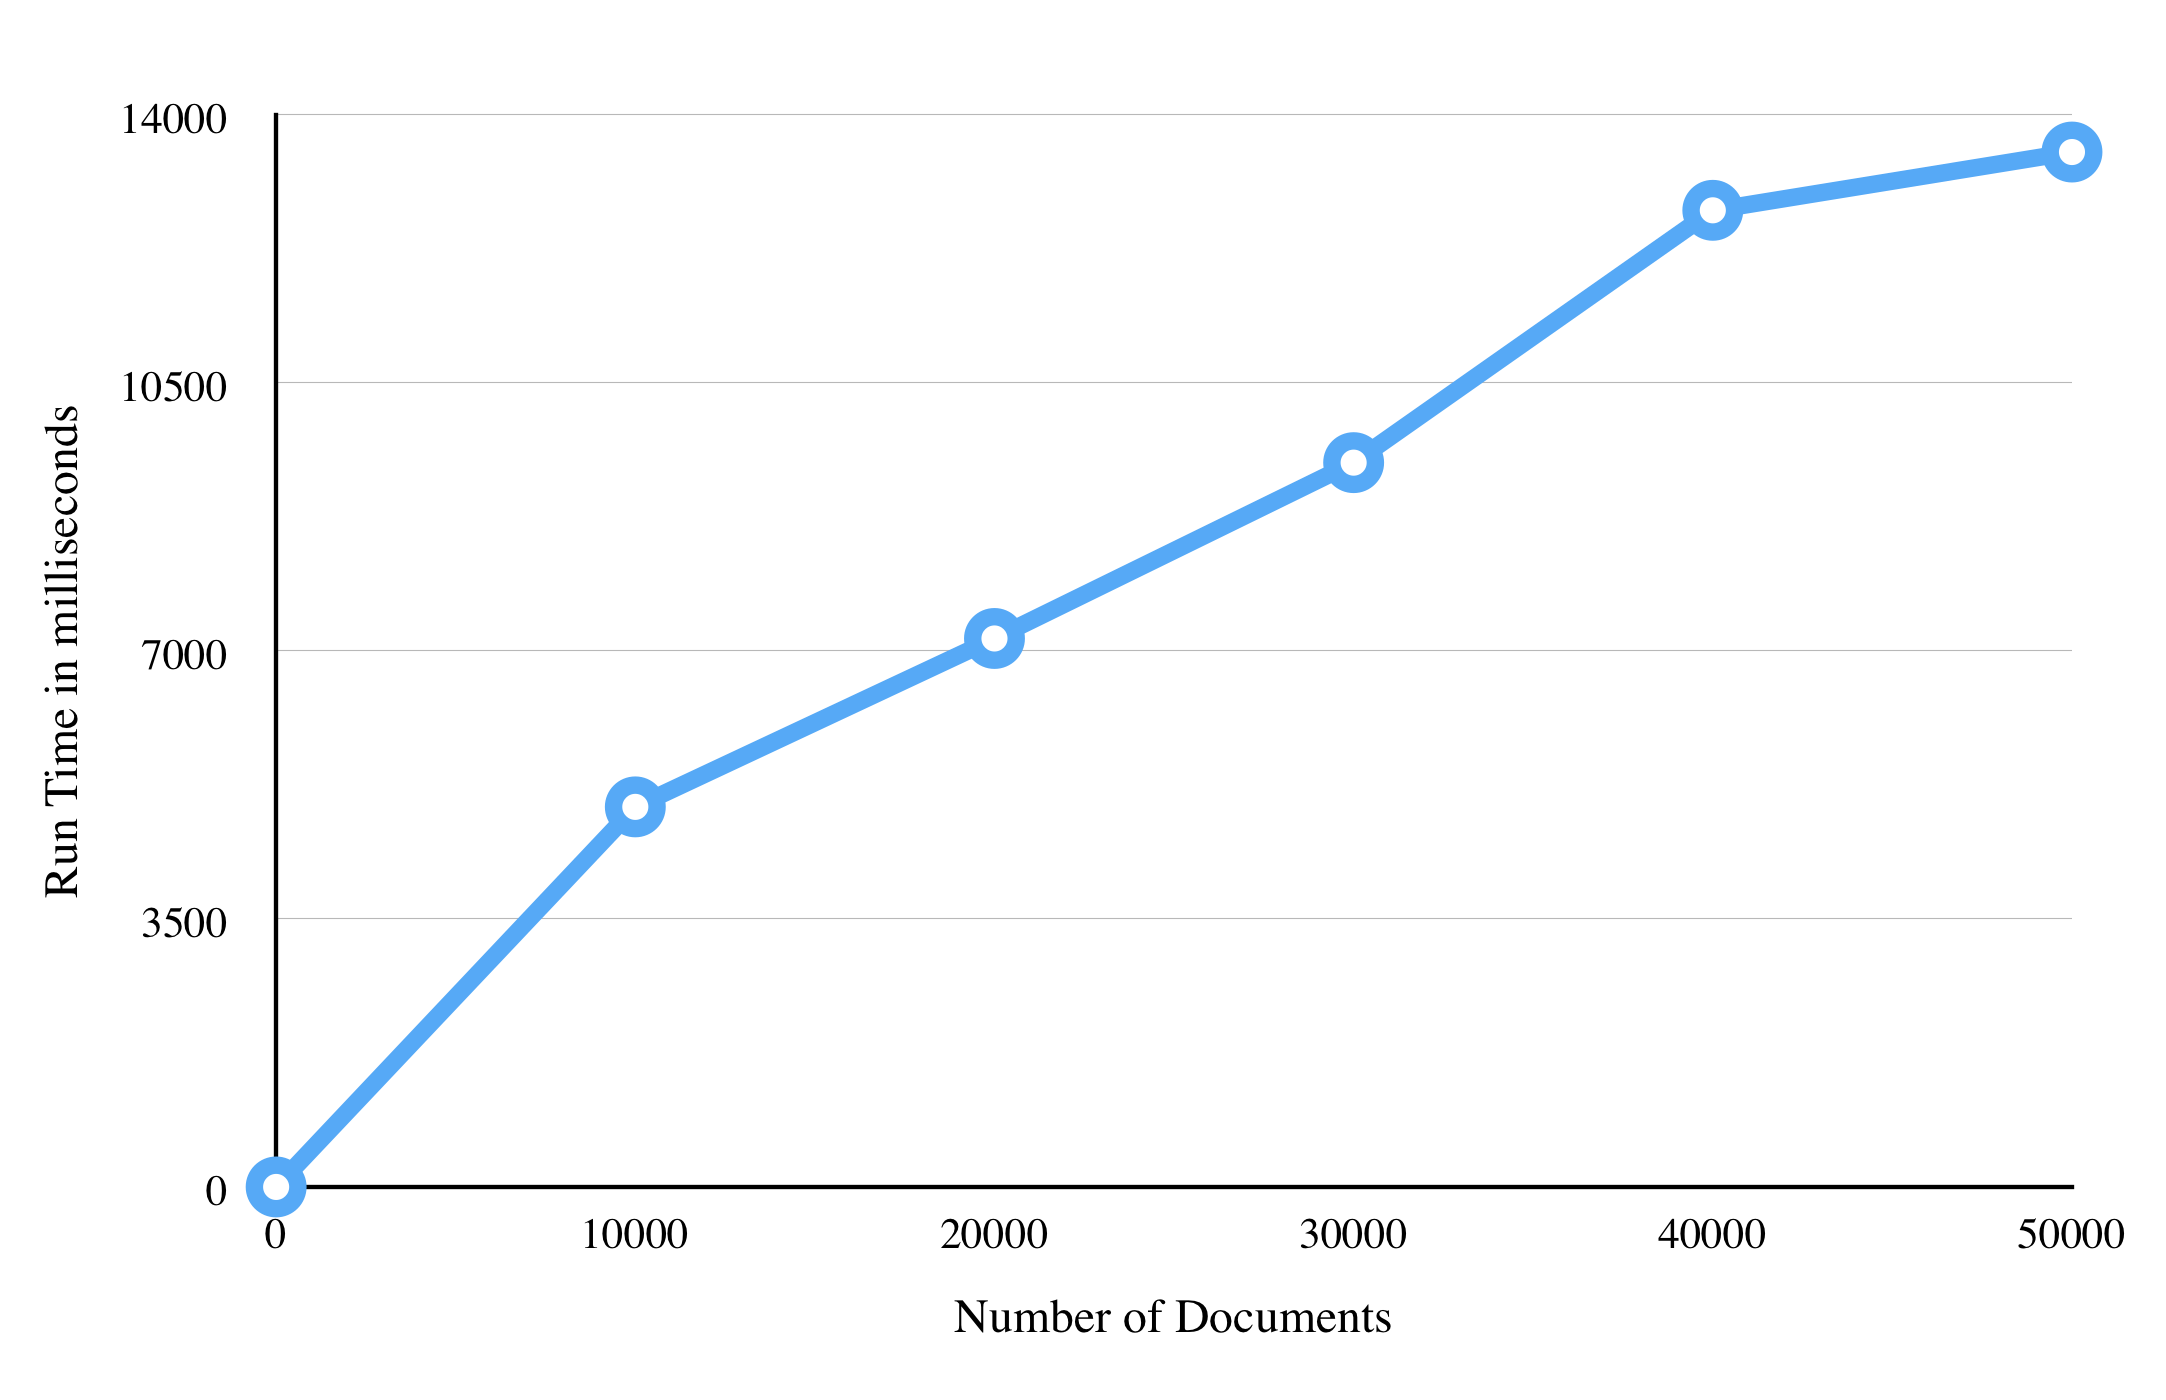
\includegraphics[keepaspectratio, width=\textwidth]{Chart.png}
		\caption{Indexing Performance}
		\label{fig:1}
	\end{figure}
\end{document}
